\documentclass[pdftex,a4paper]{scrartcl}
\usepackage[utf8]{inputenc}
\usepackage[T1]{fontenc}
\usepackage{amssymb}
\usepackage{amstext}
\usepackage{amsmath}
\usepackage{amsthm}
\usepackage{hyperref}
\usepackage{graphicx}

\title{Thoughts on Turtle Graphics with Euler Spirals}
\author{Uli Schlachter}

\newtheorem{lemma}{Lemma}
\DeclareMathOperator{\rotate}{rotate}
\DeclareMathOperator{\total}{total\_rotate}

\begin{document}

\maketitle

\section{Problem Statement}
TL;DR: \url{https://www.youtube.com/watch?v=Fx1d8x0gIu4} and \url{https://github.com/schneirob/turtlefun}.

We have an angle \(\theta\in\mathbb{R}\). For convenience, the number 1 will represent a whole rotation\footnote{I have
been told that this implies \(2\pi = 1\). Go away with your radians. :-P}. Thus, e.g. \(1/4\) represents 90° in this
representation. We now run a turtle graphics program by infinitely repeating two steps: Move forward by one unit. Rotate
by \(i\cdot\theta\), where \(i\) is the number of steps done so far.

I highly recommend the above YouTube video instead of this short descriptions. It better introduces the problem and has
pretty pictures.

The question is at which point this process becomes periodic. And whether the resulting set of points that were visit is
finite\footnote{In the video, this is referred to as returning home.} or infinite\footnote{This is called a line in the
video.}.

\section{A closer look at the visited Angles}
From the point of view of the turtle, the rotation done in step \(i\) is \(\rotate(i)=i\cdot\theta\). From the point of
view of a spectator, the rotations are cumulative. This defines \(\total(i)\) as:
\[
\total(i)=\sum_{j=1}^i \rotate(j) = \theta\cdot\sum_{j=1}^i j = \theta\cdot i\cdot(i+1)\cdot\frac{1}{2}
\]
We are curious in cases where a certain image is repeated. A certain image is repeated if the same sequence of angles
are repeated.
I.e there must be a \(o\in\mathbb{N}\) with \(o>0\) so that\footnote{This only makes sense if e.g.\ one full rotation is
equivalent to two rotations. Put differently, our angles actually live in \(\mathbb{R}/\mathbb{Z}\). See
\url{https://en.wikipedia.org/wiki/Quotient_group} if you really must. \url{https://en.wikipedia.org/wiki/Circle_group}
also seems loosely related. Surely the circle group (with multiplcaition) and \(\mathbb{R}/\mathbb{Z}\) (with addition)
are isomorphic to each other with \(x\mapsto e^{2\cdot\pi x}\).} \(\rotate(i)=\rotate(i+o)\) for all \(i\in\mathbb{N}\). Thus, we also have
\(0=\rotate(0)=\rotate(o)\) and so we are looking for cases where \(\rotate(o)\) is no rotation at all.

\section{Irrational Numbers}
For an irrational \(\theta\), \(\rotate\) cannot become periodic and the turtle will never return home.

I suppose: The resulting images will be quite chaotic and even harder to draw without falling prey to bad rounding
errors.

\section{Rational Numbers}
\(\theta\in\mathbb{Q}\) means that there are coprime \(p,q\in\mathbb{Z}\) so that \(\theta=\frac{p}{q}\). Then,
\(\rotate(q)=\theta\cdot q=p\) is the first multiple of \(\theta\) representing a whole rotation. What is the total
rotation \(\total(q)\) at this point? Insertion yields \(\total(q)=\frac{p}{q}\cdot q\cdot(q+1)\cdot \frac{1}{2}
=p\cdot(q+1)\cdot\frac{1}{2}\).
Let's do a case analysis on whether \(q\) is odd/even. But first, a Lemma.

\subsection{A Lemma}
We want to show that\footnote{Please excuse the abuse of notation. Of course, \(\rotate\) is only defined for natural
number arguments. Thus, if \(q\) is odd, \(i\) must actually be an integer plus a half.}
\(\rotate(\frac{q}{2}+i)=-\rotate(\frac{q}{2}-i)\).

We start with arguing that \(\rotate(q)=0\), i.e. is actually a multiple of full rotations and full rotations do not
influence the state\footnote{More mathematically: We are still working in \(\mathbb{R}/\mathbb{Z}\).}. By insertion,
\(\rotate(q)=\theta\cdot q=\frac{p}{q}\cdot q=p\). \(p\) is a whole number by assumption.

We now start with the right hand side of what we want to show and cleverly add zero to it:
\[
-\rotate(\frac{q}{2}-i)
=\rotate(q)-\rotate(\frac{q}{2}-i)
=\theta\cdot\left(q-(\frac{q}{2}-i)\right)
=\theta\cdot\left(\frac{q}{2}+i)\right)
=\rotate(\frac{q}{2}+i)
\]

\subsection{$q$ is even}
If \(q\) is even, then \(p\) must be odd, because we are assuming these two numbers to be coprime.
In this case\footnote{More detailed: Let \(a,b\in\mathbb{Z}\) be numbers so that \(q=2a\) and \(p=2b+1\). We have
\(\total(q)=p\cdot(q+1)\cdot\frac{1}{2}=(2b+1)\cdot(2a+1)\cdot\frac{1}{2}=2ab+a+b+\frac{1}{2}\). Everything but 1/2 is
in \(\mathbb{Z}\).}
\(\total(q)\) will be a whole number plus \(1/2\), because the product of two odd numbers is odd.

Thus, when the sequence of angles is repeated, the turtle will have turned in the opposite direction that it started
from. The next period will then draw
the same image again, but rotated by 180°. Afterwards, it will really repeat the same image again. Put differently,
after exactly \(2q\) steps does the image become repeated.

Let us look at what happens around step \(q/2\). We have \(\rotate(\frac{q}{2})=\theta\cdot \frac{q}{2}
= \frac{p}{q} \cdot \frac{q}{2} = p/2\). Since \(p\) is a whole number, this must be half a rotation, i.e.\ 180° and the
turtle turns around.

What does the turtle do after turning around?
By the lemma above, the turtle traces its steps backwards afterwards. Flipping the sign of the angle really just swaps
the meanings of "turn left" and "turn right".

What does this mean? It means that after turning around, the turtle will follow its steps backwards home! In step
q, it will arrive back at the place where it started, but turned by 180°. Then, it traces the same path in the opposite
direction and at step \(2\cdot q\) it will arrive back at its starting position with its starting angle.

\subsection{$q$ is odd}
In this case \(q+1\) is even so \(\total(q)=p\cdot\frac{q+1}{2}\) is a whole number.

Thus, when the sequence of angles is repeated, the turtle will have finished a whole number of rotations. If, and only
if, the turtle returned to its home at this point, will the set of visited points be finite.

Conjecture: These are the lines. It might be possible that the process ends up home in step \(q\), but that seems
unlikely and would produce an image that looks different than the usual images. I conjecture this does not actually
occur.

It would be interesting to see what happens around steps \(q/2-1/2\) and \(q/2+1/2\), because the lemma above still
holds. The turtle will draw the inverse of the path it did until here. There was just no 180° degree rotation like in
the case of \(q\) being even, so this does not lead back to the starting position.

\section{Taking the Position into Account}
Let us represent the position of the turtle in step \(\ell\) with \(p_\ell\in\mathbb{C}\) and its direction with
\(d_\ell\in\mathbb{C}\) with \(|d_\ell|=1\), i.e.\ \(d_\ell\) is a point on the unit circle. Then, at step \(\ell+1\), the turtle
will do:
\begin{align*}
p_{\ell+1} &= p_\ell + d_\ell &
c_{\ell+1} &= e^{(\ell+1)\cdot \theta\cdot 2\cdot \pi i} &
d_{\ell+1} &= d_ell\cdot c_{\ell+1} = d_\ell \cdot e^{\ell\cdot \theta\cdot 2\cdot \pi i}
\end{align*}
Defining \(p_0=0\) and \(d_0=1=e^0\), we can arrive at:
\[
d_\ell = e^{\theta\cdot 2\pi i\cdot \sum_{k=0}^\ell k}
= e^{\theta\cdot 2\pi i \cdot \ell\cdot(\ell+1)\frac{1}{2}}
= e^{\theta\cdot \pi i \cdot \ell\cdot(\ell+1)}
\]
This means for the position:
\[
p_\ell = \sum_{k=0}^\ell d_k
= \sum_{k=0}^\ell e^{\theta\cdot \pi i\cdot k\cdot(k+1)}
\]

Let's do some math and re-derive the Lemma above\footnote{Committing again an abuse of notation since \(c_\ell\) was
only meant to be defined for \(\ell\in\mathbb{N}\)}:
\begin{lemma}
\(c_{\frac{q}{2}-k} \cdot c_{\frac{q}{2}+k}=1\) for any \(k\in\mathbb{N}\). This means that the two rotations are
inverse to each other.
\end{lemma}
\begin{proof}
\begin{align*}
c_{\frac{q}{2}-k} \cdot c_{\frac{q}{2}+k}
&=e^{(\frac{q}{2}-k)\cdot \theta\cdot 2\cdot \pi i} \cdot e^{(\frac{q}{2}+k)\cdot \theta\cdot 2\cdot \pi i}
=e^{(\frac{q}{2}-k)\cdot \theta\cdot 2\cdot \pi i + (\frac{q}{2}+k)\cdot \theta\cdot 2\cdot \pi i}
=e^{q\cdot \theta\cdot 2\cdot \pi i} \\
&=e^{q\cdot \frac{p}{q}\cdot 2\cdot \pi i} 
=e^{p\cdot 2\cdot \pi i} 
=1^p
=1
\end{align*}
\end{proof}
Now we can show that the turtle returns to its starting orientation for odd \(q\). For even \(q\), it will face in the opposite direction.
\begin{lemma}
In general, \(d_q=(-1)^p\).
For even \(q\), this means that \(d_q=-1\).
\end{lemma}
\begin{proof}
Let us start with \(d_q\) as the product of the individual changes in directions. This product is then re-arranged into
certain combinations.
\begin{align*}
d_q
&= \prod_{\ell=0}^q c_\ell
= c_{\frac{q}{2}} \cdot \prod_{\ell=1}^{\frac{q}{2}-1} c_{\frac{q}{2}+\ell} \cdot c_{\frac{q}{2}-\ell}
\intertext{At this point the lemma can be applied and it only remains to compute \(c_{\frac{q}{2}}\):}
&= c_{\frac{q}{2}} \cdot \prod_{\ell=1}^{\frac{q}{2}-1} 1
= c_{\frac{q}{2}}
= e^{\frac{q}{2}\cdot \theta\cdot 2\cdot \pi i}
= e^{\frac{q}{2}\cdot \frac{p}{q}\cdot 2\cdot \pi i}
= e^{p\cdot \pi i}
= \left(e^{\pi i}\right)^p
= (-1)^p
\end{align*}
Since we assume that \(p\) and \(q\) are coprime, if \(q\) is even, then \(p\) must be odd. In this case, we arrive at
\(d_q=-1\). If \(q\) is odd, then \(p\) can be odd or even and we cannot conclude anything.
\end{proof}
I have no good ideas on how to continue here.

One good idea: Test whether these results actually hold. I have only derived them, but never tested them.

\section{The Continuous Case}
Instead of having two discrete steps (move forward one step, rotate, repeat), one could also consider a continuous
setting: While moving forwards, the turtle rotates at the same time. In the discrete times, the rotation increases
linearly with the number of steps. The continuous equivalent would be \(\rotate(t)=t\cdot\theta\), which leads to a
direction at time \(t\) of \(\total(t)=\int_{x=0}^t\rotate(t)\,\text{d}x=t^2\theta/2\).

More interesting is the position which is a complex number starting at \(p(0)=0\) and evolving via:
\[
\dot{p}(t) = e^{2\pi i \cdot \total(t)} = e^{\pi i \cdot t^2\theta}
\]
The author of these lines asked
\href{https://www.wolframalpha.com/input?i=p%28t%29+%3D+integrate+e%5E%28pi+*+i+*+x%5E2+*+phi%29+from+x%3D0+to+t}{Worlfram Alpha}
and got the following solution, where erf is the so-called error function\footnote{Which the author never
encountered before}:
\[
p(t) = -\frac{\sqrt[4]{-1}\;\text{erf}((-1)^{\frac{3}{4}}\sqrt{\pi}t\sqrt{\phi})}{2\sqrt{\phi}}
\]
This can now be
\href{https://www.wolframalpha.com/input?i=parametric+plot%5BReal%28-%28%28-1%29%5E%281%2F4%29+erf%28%28-1%29%5E%283%2F4%29+sqrt%28pi%29+t+sqrt%28pi%2F2%29%29%29%2F%282+sqrt%28pi%2F2%29%29%29%2C+Imag%28-%28%28-1%29%5E%281%2F4%29+erf%28%28-1%29%5E%283%2F4%29+sqrt%28pi%29+t+sqrt%28pi%2F2%29%29%29%2F%282+sqrt%28pi%2F2%29%29%29%5D+for+t%3D0..20}{plotted},
for example with \(\phi=90^\circ=\pi/2\) and \(t\) from 0 to 1, and then from 0 to 20:

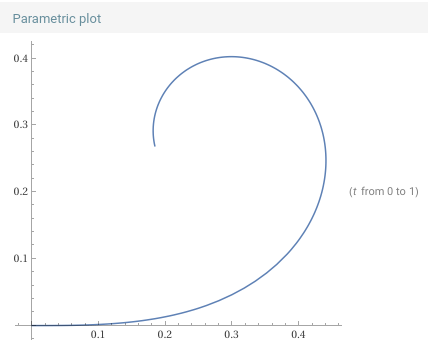
\includegraphics[width=\textwidth]{continuous1.png}

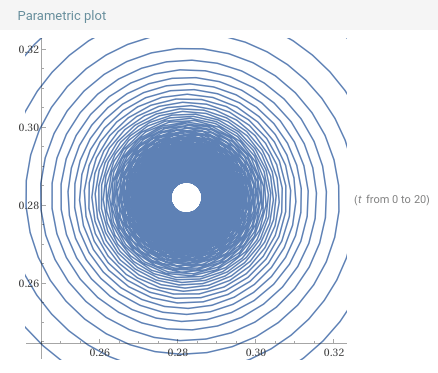
\includegraphics[width=\textwidth]{continuous20.png}

\section{Acknowledgements}
Thanks a lot to Schneirob for producing \url{https://www.youtube.com/watch?v=Fx1d8x0gIu4}. This made it really easy for
me to get an overview over things and identify some interesting angels. Then I used
\url{https://github.com/schneirob/turtlefun} to get the angles that occur during the Euler spiral. All the hard parts
were already prepared for me.

\end{document}
